\subsection{Consensus group} \label{sec:assign_group}

\begin{figure}[!htb]
	\centering
	\begin{tikzpicture}[genericStyle, every node/.style={circle, draw, minimum size=1.7em, text width=1em, align=center, inner sep=0pt}]
    \def\UVsep{2.5em}
    \def\colSep{3em}
    \def\rowSep{1.2em}
    \def\hStep{0.7em}

    % Figure 1
    \node[nodeUStyle] (a1) at (0,0) {$u_i$};
    \node[nodeUStyle] (a2) [below=\hStep of a1] {$u_j$};
    \node[nodeVStyle, right=\UVsep of a1] (b1) {$v_i$};
    \node[nodeVStyle, right=\UVsep of a2] (b2) {$v_j$};

    \draw[graphEdgeStyle] (a1) -- (b1); 
    \draw[graphEdgeStyle] (a2) -- (b2);

    \coordinate (midA) at ($(a1.south)!0.5!(a2.north)$);
    \node[draw=none, left=0.4em of midA]
    {$\Big\updownarrow$};

    \node[nodeUStyle, right=\colSep of b1] (c1) {$u_i$};
    \node[nodeUStyle, right=\colSep of b2] (c2) {$u_j$};
    \node[nodeVStyle, right=\UVsep of c1] (d1) {$v_i$};
    \node[nodeVStyle, right=\UVsep of c2] (d2) {$v_j$};

    \draw[graphEdgeStyle] (c1) -- (d2); 
    \draw[graphEdgeStyle] (c2) -- (d1);

    \coordinate (midB) at ($(b1.east)!0.5!(b2.east)$); 
    \coordinate (midC) at ($(c1.west)!0.5!(c2.west)$);
    \coordinate (midBC) at ($(midB)!0.5!(midC)$);
    \node[draw=none, text width=2em] at (midBC) {$\Longleftrightarrow$};  

    % Figure 2
    \node[nodeUStyle] (a3) [below=\rowSep of a2] {};
    \node[nodeUStyle] (a4) [below=\hStep of a3] {};

    \coordinate (midA2) at ($(a3.south)!0.5!(a4.north)$);
    \node[draw=none, left=0.4em of midA2]
    {$\Big\updownarrow$};

    \coordinate (midA3) at ($(a3.east)!0.5!(a4.east)$);
    \node[nodeVStyle, right=\UVsep of midA3] (b3) {};
    \draw[graphEdgeStyle] (a3) -- (b3);
    \draw[graphEdgeStyle] (a4) -- (b3);

    \node[nodeUStyle, below=\rowSep of c2] (c3) {};
    \node[nodeUStyle, below=\hStep of c3] (c4) {};

    \coordinate (midC3) at ($(c3.east)!0.5!(c4.east)$);
    \node[nodeVStyle, right=\UVsep of midC3] (d3) {};
    \draw[graphEdgeStyle] (c3) -- (d3);
    \draw[graphEdgeStyle] (c4) -- (d3);

    \coordinate (midC2) at ($(c3.west)!0.5!(c4.west)$);
    \coordinate (midBC2) at ($(b3.east)!0.5!(midC2)$);
    \node[draw=none, text width=2em] at (midBC2) {$\Longleftrightarrow$};  
\end{tikzpicture}

	%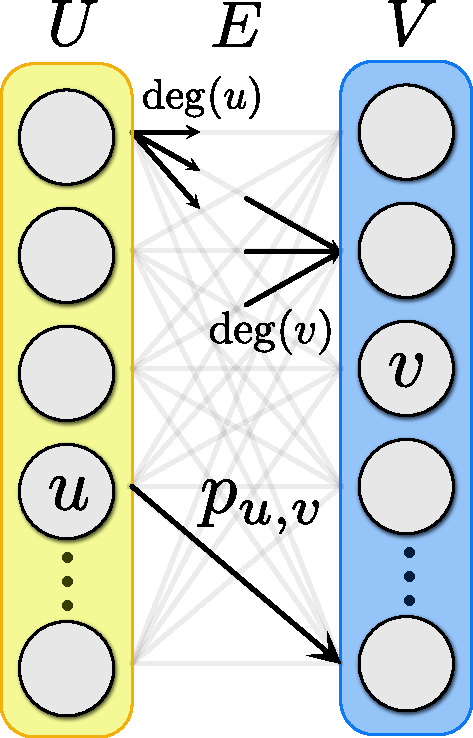
\includegraphics[width=0.4\columnwidth]{figs/bipartite_map.pdf}
	\caption{\textbf{Swap symmetry.}???.}\label{fig:swap_symmetry}
\end{figure}

* Space of satisfying graph assignments is given by the action of the consensus group on any valid graph assignment,
\begin{align}
	\{\mathcal{G}\} = C_d \times \mathcal{G}_{n,d}.
\end{align}

* Clarify edge transformations rather than U and V.

* Permutation group

* Graph automorphisms not the same as automorphisms over edges.

* Automorphism group in edge space describes invariances. Sym/Aut gives consensus group?

* Automorphism group over edge permutations is in general inequivalent to the conventional definition of a graph automorphism: for $\mathcal{G}=(V,E)$, $(u,v)\in E \Leftrightarrow (\sigma(u),\sigma(v))\in E$ %$\mathrm{Aut}(\mathcal{G}): $

* Counting graph automorphisms is known to be

* While all permutations within $E_U$ and $E_V$ are degree preserving, not all are unique.

Transformations over the space of satisfying graph realisations of given degree sequence, $d$, defines the \emph{consensus group}, $C(d)$, fully characterised by its degree sequence. Over the space of satisfying graphs the consensus group,
\begin{align}
	\phi: C(d)\times \mathcal{G}_d \to \mathcal{G}_d,
\end{align}
is identically the symmetric group,
\begin{align}
	\phi: C(d) = \mathrm{Sym}(\mathcal{G}_d).
\end{align}
The action of the consensus group may be equivalently defined via permutations within the columns of satisfying edge-sets,
\begin{align}
	\psi: C(d)\times (E_U\times E_V) \to (E_U\times E_V),
\end{align}
the group of non-degenerate permutations within the columns of $E$, which discounts permutations under which edge-sets remain invariant, a subgroup of the symmetric group acting on either column, both of length $|E|$,
\begin{align}
	(\psi, E_{U,V}) & \subseteq S_{|E|}.
\end{align}

In the special case of 1-regular graphs, satisfying consensus assignments define bijective maps across graph partitions and the group action over edge-set columns is identically the symmetric group,
\begin{align}
	\psi: C(d) = S_{|E|},\,\delta(\mathcal{G})=\Delta(\mathcal{G})=1,
\end{align}
as there are no degenerate permutations.

Hence, the order of the consensus group, equivalently the number of unique consensus assignments, is upper-bounded by the order of the symmetric group acting on edge-sets, $S_{|E|}$,
\begin{align} \label{eq:orbit_order}
	%|C(d)| &= \frac{|E|!}{\prod_{u\in U}\mathrm{deg}(u)!\cdot \prod_{v\in V}\mathrm{deg}(v)!} \nonumber\\
	%&= \binom{|E|!}{d_1,\dots,d_{|U|+|V|}} \nonumber\\
	|C(d)| & \leq |E|!,
\end{align}
with equality when \mbox{$\Delta(\mathcal{G})=1$}.

Employing element-wise inequality notation for degree sequences, of equal length, \mbox{$|d|=|d'|$},
\begin{align}
	d' < d \coloneqq d'_i < d_i,\, \forall\, i,
\end{align}
affords the equivalent relations between degree sequences, satisfying assignment graphs and their respective subgroup structures,
\begin{align} \label{eq:sub_dgc}
	d' < d & \Rightarrow \mathcal{G}_{d'} \subset \mathcal{G}_d \Rightarrow C(d') \triangleleft C(d),
\end{align}
where $C(d')$ is a normal subgroup of $C(d)$ and $\mathcal{G}_{d'}$ is a subgraph of $\mathcal{G}_d$ under edge-removal.

%Consensus groups exhibit a recursive normal subgroup structure,
%\begin{align}
%	C(d') &\triangleleft C(d),
%\end{align}
%reflecting the associated subgraph structure,
%\begin{align}
%	\mathcal{G}' &\subset \mathcal{G}.
%\end{align}

%As edge exchange operations are symmetric across $U$ and $V$ the consensus group may equivalently be associated with the space of edge permutations on either. Despite having support over vertex sets with distinct degree sequences they afford the same space of edge permutations.

The number of bits required to uniquely address the group's orbit scales as (Fig.~\ref{fig:bits_permutations}),
\begin{align}
	n & = \log_2(|\mathrm{Orb}_C(E)|) \leq \log_2(|E|!).
\end{align}

\subsubsection{Generalised Fisher-Yates shuffle for finite groups}

The Fisher-Yates shuffle may be generalised to uniformly sample over other finite groups (Alg.~\ref{alg:fisher_yates_general}).

Alg.~\ref{alg:fisher_yates} may be interpreted as follows: for every index $i$ the associated value $v_i$ is chosen uniformly from the set of unassigned values $v_j$ (where $0\leq j\leq i$). More generally, we would choose $v_i$ uniformly from the set of elements it is allowed to transition to under the action of the respective group. For the symmetric group, $S_n$, this includes all elements, whereas other groups in general constrain the set of allowed transitions.

Consider a group $G$ defined over set $X$,
\begin{align}
	\phi: G\times X \to X.
\end{align}
Elements of the set $x\in X$ individually transform under the group action of $G$ to their orbit,
\begin{align}
	\mathrm{Orb}_G(x) & = G\times x \nonumber                                         \\
	                  & = \{ y\in X \,\,|\,\, \exists \,g\in G \,\,|\,\, y=g\cdot x\}
\end{align}
defining sets for the allowed transitions of $x$ under the action of $G$. For the symmetric group we have,
\begin{align}
	\mathrm{Orb}_{S_n}(x) = X,
\end{align}
as all elements may map to all others, while for other groups the orbit of $x$ may be a subset of elements.

We define the \emph{transition set}, $t$, to be the set of allowed transitions of $x$ under the group action of $G$, given by the intersection unassigned elements ($s$) and the orbit of $x$,
\begin{align}
	t = \mathrm{Orb}_G(x) \cap s.
\end{align}

%Sattolo's algorithm for uniformly sampling the cyclic group defines the transition set to include all unassigned elements excluding element $i$. This arises because under a cyclic permutation all elements must permute

\begin{algorithm}[H]
	\begin{algorithmic}
		\Function{GroupShuffle}{$\vec{v}$, $G$} $\to \vec{v}$\Comment{$O(n^2)$}
		\For{$i \gets |\vec{v}|-1 \textbf{ to } 1$} \Comment{$O(n)$}
		\State $s \gets \{\vec{v}_j\,|\, 0\leq j\leq i\}$ \Comment{Unassigned elements}
		\State $t \gets \textsc{TransitionSet}(\vec{v}_i,s,G)$ \Comment{$O(n)$}
		\State $j \gets \textsc{Random}(t)$ \Comment{$O(1)$}
		\State $v_i\leftrightarrow v_j$ \Comment{Exchange}
		\EndFor
		\State \Return $\vec{v}$
		\EndFunction
		\\
		\Function{TransitionSet}{$x$, $s$, $G$} $\to t$ \Comment{$O(n)$}
		\State \Return $(G\times x) \cap s$ \Comment{Group action on reduced set}
		\EndFunction
	\end{algorithmic}
	\caption{Generalised Fisher-Yates shuffle for finite groups $G$.}\label{alg:fisher_yates_general}
\end{algorithm}

\textbf{WRONG FOR THE CONSENSUS GROUP:} The uniqueness of execution paths in the generalised algorithm follows the same argument as for the the original scheme. The probability associated with an execution path is,
\begin{align} \label{eq:group_order_shuffle}
	P(\vec{d}) & = \prod_{i=1}^{n} p(\vec{d}_i) = \prod_{i=1}^{n} \frac{1}{|t_i|} = \prod_{i=1}^{n} \frac{1}{|\mathrm{Orb}_{G^{(i)}}(x_i)|},
\end{align}
where \mbox{$\vec{d}_i=1/|t_i|$} is the probability of making choice \mbox{$j=\vec{d}_i$} at level $i$ under uniform sampling, and $G^{(i)}$ denotes the $i$th level subgroup of $G=G^{(n)}$ acting on the reduced set predicated on the removal of already assigned elements of $X$,
\begin{align} \label{eq:subgroup_struct}
	G^{(i)}   & \times X^{(i)} \to X^{(i)},\nonumber   \\
	X^{(i)}   & = X\backslash\{x_{k}\}_{k>i},\nonumber \\
	G^{(i-1)} & \triangleleft G^{(i)},
\end{align}
defining a composition series followed by the algorithm to iteratively assign set elements,
\begin{align}
	1 = G^{(0)} \triangleleft \cdots \triangleleft G^{(n-1)} \triangleleft G^{(n)} = G,
\end{align}
where each subgroup acts on the set predicated on the removal of an element from the set upon which the supergroup acts.

As the consensus group is both free\footnote{Free groups: all elements are invariant under the action of all group elements except the identity,
	\begin{align}
		g\cdot x = x\, \Rightarrow\, g=e.\nonumber
	\end{align}} and transitive\footnote{Transitive groups: all elements $x\in X$ map to all elements $y\in X$ under the action of some group element $g\in G$,
	\begin{align}
		x,y\in X \,|\, \exists\, g\in G \,\,|\,\, g\cdot x=y.\nonumber
	\end{align}}
it has regular\footnote{Regular group action: $\forall\,\,x,y\in X \,\,|\,\, g\cdot x=y$, $g\in G$ is unique.} group action and all group elements have the same orbit. Hence, $|t_i|$ is level-dependent on $i$ but independent of group element $x\in X$ and execution pathway $l\in\mathcal{L}$. $P(\vec{d})$ is therefore a function of the group but uniform across all group elements.

\subsubsection{Uniformly sampling the consensus group (old)}

Uniformly sampling the consensus group is achieved by defining transition sets as per Alg.~\ref{alg:consensus_shuffle}, whereby allowed transitions under edge exchanges \mbox{$v_i\leftrightarrow v_j$} satisfy the Boolean constraint,
\begin{align}
	[(u_i,v_j) \not\in E] \lor [(u_j,v_i)	\not\in E] = 1,
\end{align}
requiring that newly created edges not be previously existing ones. ??? CHECK

An \mbox{$v_i\leftrightarrow v_j$} exchange within edge-set $E$ is equivalent to eliminating existing edges,
\begin{align}
	e_i = (u_i,v_i),\,\, e_j = (u_j,v_j),
\end{align}
and replacing them with permuted edges,
\begin{align}
	e_i' = (u_i,v_j),\,\, e_j' = (u_j,v_i).
\end{align}
Thus, edge-set invariance under \mbox{$v_i\leftrightarrow v_j$} requires,
\begin{align}
	E \backslash \{e_i,e_j\} \cup \{e_i',e_j'\} = E,
\end{align}
which implies,
\begin{align}
	\{e_i',e_j'\}            & \in E,\nonumber                        \\
	E \backslash \{e_i,e_j\} & = E \backslash \{e_i',e_j'\},\nonumber \\
	\{e_i,e_j\}              & =\{e_i',e_j'\}.
\end{align}
Hence, the requirement exchanges \mbox{$v_i\leftrightarrow v_j$} not be edge-set invariant is,
\begin{align}
	\{e_i',e_j'\}            & \in E,\nonumber                        \\
	E \backslash \{e_i,e_j\} & = E \backslash \{e_i',e_j'\},\nonumber \\
	\{e_i,e_j\}              & =\{e_i',e_j'\}.
\end{align}

%\begin{align}
%	E \backslash \{e_i,e_j\} = E \backslash \{e_i',e_j'\}.
%\end{align}

%As the edge-sets of simple graphs are simple sets, 

%
%* The exchange operation $v_i\leftrightarrow v_j$ prospectively creates the new edges $(u_i,v_j)$ and $(u_j,v_i)$. If either already exist this would either: violate $\mathcal{G}$ being a simple graph; constitute a degenerate edge permutation. Hence, 

* Need to clarify notation here. $i$ here refers to index in $E$, but usually we use it for a node number.

%\begin{align} \label{eq:exchange_rule}
%		(u_i \neq u_j) \odot (v_i \neq v_j) = 1,
%\end{align}
%where $\odot$ denotes logical XNOR. This constraint is equivalent to,
%\begin{align}
%		[(u_i \neq u_j) \land (v_i \neq v_j)] \lor [(u_i = u_j) \land (v_i = v_j)] = 1,
%\end{align}
%where the first clause allows exchange operations between nodes $u_i$ and $u_j$, equivalently between consensus sets $v_i$ and $v_j$, only when distinct (Fig.~\ref{fig:swap_sym}), and the second clause is equivalent to $i=j$, ensuring inclusion of $u_i$ itself.

%\begin{figure}[!htb]
%\centering
%\begin{tikzpicture}[genericStyle, every node/.style={circle, draw, minimum size=1.7em, text width=1em, align=center, inner sep=0pt}]
    \def\UVsep{2.5em}
    \def\colSep{3em}
    \def\rowSep{1.2em}
    \def\hStep{0.7em}

    % Figure 1
    \node[nodeUStyle] (a1) at (0,0) {$u_i$};
    \node[nodeUStyle] (a2) [below=\hStep of a1] {$u_j$};
    \node[nodeVStyle, right=\UVsep of a1] (b1) {$v_i$};
    \node[nodeVStyle, right=\UVsep of a2] (b2) {$v_j$};

    \draw[graphEdgeStyle] (a1) -- (b1); 
    \draw[graphEdgeStyle] (a2) -- (b2);

    \coordinate (midA) at ($(a1.south)!0.5!(a2.north)$);
    \node[draw=none, left=0.4em of midA]
    {$\Big\updownarrow$};

    \node[nodeUStyle, right=\colSep of b1] (c1) {$u_i$};
    \node[nodeUStyle, right=\colSep of b2] (c2) {$u_j$};
    \node[nodeVStyle, right=\UVsep of c1] (d1) {$v_i$};
    \node[nodeVStyle, right=\UVsep of c2] (d2) {$v_j$};

    \draw[graphEdgeStyle] (c1) -- (d2); 
    \draw[graphEdgeStyle] (c2) -- (d1);

    \coordinate (midB) at ($(b1.east)!0.5!(b2.east)$); 
    \coordinate (midC) at ($(c1.west)!0.5!(c2.west)$);
    \coordinate (midBC) at ($(midB)!0.5!(midC)$);
    \node[draw=none, text width=2em] at (midBC) {$\Longleftrightarrow$};  

    % Figure 2
    \node[nodeUStyle] (a3) [below=\rowSep of a2] {};
    \node[nodeUStyle] (a4) [below=\hStep of a3] {};

    \coordinate (midA2) at ($(a3.south)!0.5!(a4.north)$);
    \node[draw=none, left=0.4em of midA2]
    {$\Big\updownarrow$};

    \coordinate (midA3) at ($(a3.east)!0.5!(a4.east)$);
    \node[nodeVStyle, right=\UVsep of midA3] (b3) {};
    \draw[graphEdgeStyle] (a3) -- (b3);
    \draw[graphEdgeStyle] (a4) -- (b3);

    \node[nodeUStyle, below=\rowSep of c2] (c3) {};
    \node[nodeUStyle, below=\hStep of c3] (c4) {};

    \coordinate (midC3) at ($(c3.east)!0.5!(c4.east)$);
    \node[nodeVStyle, right=\UVsep of midC3] (d3) {};
    \draw[graphEdgeStyle] (c3) -- (d3);
    \draw[graphEdgeStyle] (c4) -- (d3);

    \coordinate (midC2) at ($(c3.west)!0.5!(c4.west)$);
    \coordinate (midBC2) at ($(b3.east)!0.5!(midC2)$);
    \node[draw=none, text width=2em] at (midBC2) {$\Longleftrightarrow$};  
\end{tikzpicture}

%%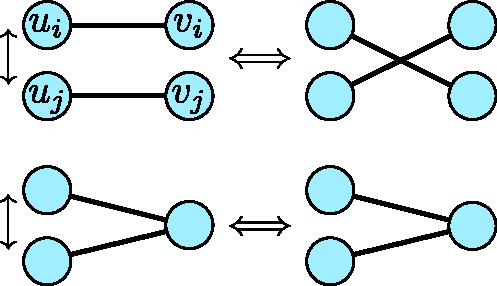
\includegraphics[width=0.5\columnwidth]{figs/swap_symmetry.pdf}
%\caption{\textbf{Degeneracy rule for vertex exchanges in the consensus group.} Allowed vertex exchanges $u_i\leftrightarrow u_j$ (equivalently $v_i\leftrightarrow v_j$) require vertices in both the $U$ and $V$ partitions of the bipartite graph to be distinct, as per Eq.~\eqref{eq:exchange_rule}.} \label{fig:swap_sym}	
%\end{figure}

\begin{algorithm}[H]
	\begin{algorithmic}
		\Function{ConsensusShuffle}{$\mathcal{X}$, $\vec{u}$, $\vec{v}$} $\to \vec{v}$ \Comment{$O(n^2)$}
		\For{$i \gets |\vec{v}|-1 \textbf{ to } 1$} \Comment{$O(n)$}
		\State $t \gets \{0\leq k< i \,|\, \textsc{Transition}(i,k) = 1\}$ \Comment{$O(n)$}
		\State $j \gets \textsc{Random}(\mathcal{X}, t \cup i)$ \Comment{$O(1)$}
		\State $v_i\leftrightarrow v_j$ \Comment{Exchange}
		\EndFor
		\State \Return $\vec{v}$
		\EndFunction
		\\
		\Function{AllowTransition}{$i$, $j$} $\to \{0,1\}$ \Comment{$O(n)$}
		\State \Return $[(u_i,v_j) \notin E] \land [(u_j,v_i) \notin E]$
		\EndFunction
	\end{algorithmic}
	\caption{The transition set for the consensus group may be characterised by the constraints imposed by the group relations characterising non-degenerate transitions. The \textsc{Transition} function is a binary operator specifying whether index $j$ is an allowed transition for index $i$, defining the respective transition set.}\label{alg:consensus_shuffle}
\end{algorithm}

The regular action of the consensus group implies that under symmetrisation via uniform sampling all satisfying edge assignments $\{E\}$ occur with equal probability, from which it follows,
% It follows that every node $u$ will be ass, and nodes are assigned with uniform probability to all consensus sets, and every consensus set has uniform probability of comprising any subset of nodes,
\begin{align} \label{eq:prob_cons}
	p_{u,v}                       & = \frac{\mathrm{deg}(u)}{|V|},\nonumber \\
	\sum_{v\in V} p_{u,v}         & = \mathrm{deg}(u),\nonumber             \\
	\sum_{u\in U} p_{u,v}         & = 1, \nonumber                          \\
	\sum_{u\in U, v\in V} p_{u,v} & = |E|,
\end{align}
where $p_{u,v}$ is the probability of node $u$ being assigned to consensus set $v$.
* Regular action.

* Use uniform bidding to preserve average case $r$. If non-uniform the effective $r$ in consensus sets is biased towards the $r$ of higher bidders.

* ???
* For a given edge $e=(u,v)$ in edge-set $e\in E$, the order of the orbit of vertex $v$ under the group action $\psi$ is,
\begin{align}
	\psi: |\mathrm{Orb}_C(v)| & = |V/v| = |V|-1.
\end{align}
That is, vertex $v$ may permute to any vertex other than itself.

* ??? TODO. Fig.~\ref{fig:bipartite_map}

* Bipartite decomposition or bipartite dimension. Edge-disjoint union of complete bipartite graphs or bicliques.

* Degree-preserving biclique decomposition.

* Kmn defines invariant subgraphs under edge-permutation. Vertices within a Kmn subgraph define graph automorphisms under vertex permutations $\sigma$.
\begin{align}
	\varphi: (u,v)\in E \Longleftrightarrow (\sigma_u,\sigma_v)	\in E.
\end{align}

For complete graphs all vertex permutations within each bipartition define graph automorphisms,
\begin{align}
	\mathrm{Aut}(K_{m,n}) = S_m\times S_n.
\end{align}


* Graph sum (disjoint union)
\begin{align}
	\mathcal{G}_d^{(K)} = \bigoplus_{b} K_{m_b,n_b}.
\end{align}

* Not all graphs can be decomposed this way. Determining this is NP-hard in general.

For $K_{m,n}$,
\begin{align}
	\mathrm{deg}(u) & =n,\,\forall\, u\in U,\nonumber \\
	\mathrm{deg}(v) & =m,\,\forall\, v\in V.
\end{align}

* Admits graph automorphisms,
\begin{align}
	\bigtimes_{b} (S_{m_b}\times S_{n_b}) \subseteq \mathrm{Aut}(\mathcal{G}_d^{(K)}).
\end{align}
* Is it equality?

\begin{figure}[!htb]
	\begin{tikzpicture}[genericStyle]
    \def\Km{5}
    \def\Kn{4}
    \def\Kmskip{4}
    \def\Knskip{3}
    \def\voff{-0.575}
    \def\dotsoff{0.15}
    \def\UVsep{2.8}
    
    \foreach \i in {1,...,\Km} {
        \ifnum\i=\Kmskip
          \node[draw=none] (a\i) at (0,\dotsoff-\i) {\LARGE $\vdots$};
        \else
            \ifnum\i=\Km
                \node[nodeUStyle] (a\i) at (0,-\i) {$u_m$};
            \else
                \node[nodeUStyle] (a\i) at (0,-\i) {$u_{\i}$};
            \fi
        \fi
    }
    \foreach \i in {1,...,\Kn} {
        \ifnum\i=\Knskip
            \node[draw=none] (b\i) at (\UVsep,\dotsoff+\voff-\i) {\LARGE $\vdots$};
        \else
            \ifnum\i=\Kn
                \node[nodeVStyle] (b\i) at (\UVsep,\voff-\i) {$v_n$};
            \else
                \node[nodeVStyle] (b\i) at (\UVsep,\voff-\i) {$v_{\i}$};
            \fi
        \fi
    }
    
    \foreach \i in {1,...,\Km} {
        \foreach \j in {1,...,\Kn} {
        \ifnum\i=\Kmskip
        \else
            \ifnum\j=\Knskip
            \else
                \draw[graphEdgeStyle] ($(a\i.east)$) -- ($(b\j.west)$);
            \fi
        \fi
        }
    }

    \node[draw=none] at ($(a1)!0.5!(b1) + (0,0.5)$) {$K_{m,n}$};
\end{tikzpicture}
	\caption{\textbf{Complete bipartite graph, $K_{m,n}$.} Vertices in each bipartition have uniform degree.} \label{fig:K_mn_graph}
\end{figure}

\begin{figure}[!htb]
	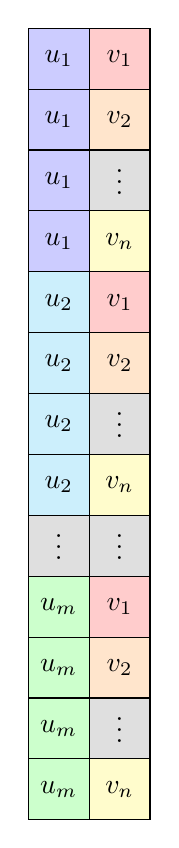
\begin{tikzpicture}
  \tikzset{square node/.style={draw, minimum size=2.2em}}

    \definecolor{verylightgray}{rgb}{0.9, 0.9, 0.9}
    \colorlet{color1}{blue!20}
    \colorlet{color2}{cyan!20}
    \colorlet{color3}{green!20}

    \colorlet{colorA}{red!20}
    \colorlet{colorB}{orange!20}
    \colorlet{colorC}{yellow!20}

  \def\x{2.2em}

    % 1
    \node[square node, fill=color1] at (\x,-\x) {$u_1$};
    \node[square node, fill=colorA] at (2*\x,-\x) {$v_1$};

    \node[square node, fill=color1] at (\x,-2*\x) {$u_1$};
    \node[square node, fill=colorB] at (2*\x,-2*\x) {$v_2$};
    
    \node[square node, fill=color1] at (\x,-3*\x) {$u_1$};
    \node[square node, fill=lightgray!50] (d1) at (2*\x,-3*\x) {};
    \node[draw=none] at (d1) [yshift=0.25em] {$\vdots$};

    \node[square node, fill=color1] at (\x,-4*\x) {$u_1$};
    \node[square node, fill=colorC] at (2*\x,-4*\x) {$v_n$};

     % 2
    \node[square node, fill=color2] at (\x,-5*\x) {$u_2$};
    \node[square node, fill=colorA] at (2*\x,-5*\x) {$v_1$};

    \node[square node, fill=color2] at (\x,-6*\x) {$u_2$};
    \node[square node, fill=colorB] at (2*\x,-6*\x) {$v_2$};
    
    \node[square node, fill=color2] at (\x,-7*\x) {$u_2$};
    \node[square node, fill=lightgray!50] (d2) at (2*\x,-7*\x) {};
    \node[draw=none] at (d2) [yshift=0.25em] {$\vdots$};

    \node[square node, fill=color2] at (\x,-8*\x) {$u_2$};
    \node[square node, fill=colorC] at (2*\x,-8*\x) {$v_n$};

    % ...
    \node[square node, fill=lightgray!50] (d3) at (\x,-9*\x) {};
    \node[draw=none] at (d3) [yshift=0.25em] {$\vdots$};
    \node[square node, fill=lightgray!50] (d4) at (2*\x,-9*\x) {};
    \node[draw=none] at (d4) [yshift=0.25em] {$\vdots$};

    % m
    \node[square node, fill=color3] at (\x,-10*\x) {$u_m$};
    \node[square node, fill=colorA] at (2*\x,-10*\x) {$v_1$};

    \node[square node, fill=color3] at (\x,-11*\x) {$u_m$};
    \node[square node, fill=colorB] at (2*\x,-11*\x) {$v_2$};
    
    \node[square node, fill=color3] at (\x,-12*\x) {$u_m$};
    \node[square node, fill=lightgray!50] (d5) at (2*\x,-12*\x) {};
    \node[draw=none] at (d5) [yshift=0.25em] {$\vdots$};

    \node[square node, fill=color3] at (\x,-13*\x) {$u_m$};
    \node[square node, fill=colorC] at (2*\x,-13*\x) {$v_n$};

\end{tikzpicture}
	\caption{\textbf{Canonically ordered edge-set for complete bipartite graph, $K_{m,n}$.}} \label{fig:K_mn_edges}
\end{figure}

\begin{figure}[!htb]
	\centering
	\begin{minipage}[t]{0.4\columnwidth}
		\begin{tikzpicture}[genericStyle]
    \def\UVsep{2.5}
    \def\vMult{1.8}
    
    \colorlet{color1}{blue}
    \colorlet{color2}{cyan}
    \colorlet{color3}{green}
    \colorlet{colorA}{red}
    \colorlet{colorB}{orange}
    \colorlet{colorC}{yellow}
    
    \node[draw=color1, fill=color1!20, myShadow] (a1) at (0,-1*\vMult) {$u_1$};
    \node[draw=color2, fill=color2!20, myShadow] (a2) at (0,-2*\vMult) {$u_2$};
    \node[draw=color3, fill=color3!20, myShadow] (a3) at (0,-3*\vMult) {$u_3$};
    
    \node[draw=colorA, fill=colorA!20, myShadow] (b1) at (\UVsep,-1*\vMult) {$v_1$};
    \node[draw=colorB, fill=colorB!20, myShadow] (b2) at (\UVsep,-2*\vMult) {$v_2$};
    \node[draw=colorC, fill=colorC!20, myShadow] (b3) at (\UVsep,-3*\vMult) {$v_3$};
    
     \foreach \i in {1,...,3} {
     	\foreach \j in {1,...,3} {
        	\draw[graphNonEdgeStyle] ($(a\i.east)$) -- ($(b\j.west)$);
        }
    }
    
    \draw[graphEdgeStyle] ($(a1.east)$) -- ($(b1.west)$);
    \draw[graphEdgeStyle] ($(a1.east)$) -- ($(b2.west)$);
    \draw[graphEdgeStyle] ($(a2.east)$) -- ($(b2.west)$);
    \draw[graphEdgeStyle] ($(a2.east)$) -- ($(b3.west)$);
    \draw[graphEdgeStyle] ($(a3.east)$) -- ($(b3.west)$);
    \draw[graphEdgeStyle] ($(a3.east)$) -- ($(b1.west)$);
    
    \node[draw=none] at ($(a1)!0.5!(b1) + (0,0.75)$) {$\mathcal{G}_{3,2}$};
\end{tikzpicture}
	\end{minipage}
	\quad
	\begin{minipage}[t]{0.3\columnwidth}
		\begin{tikzpicture}
  \tikzset{square node/.style={draw, minimum size=2.2em}}
  \colorlet{color1}{blue}
  \colorlet{color2}{cyan}
  \colorlet{color3}{green}

  \colorlet{colorA}{red}
  \colorlet{colorB}{orange}
  \colorlet{colorC}{yellow}

  \def\x{2.2em}

  \node[square node, fill=color1!20] (u1) at (\x,-\x) {$u_1$};
  \node[square node, fill=colorA!20] (v1) at (2*\x,-\x) {$v_1$};
  \node[square node, fill=color1!20] at (\x,-2*\x) {$u_1$};
  \node[square node, fill=colorB!20] at (2*\x,-2*\x) {$v_2$};

  \node[square node, fill=color2!20] at (\x,-3*\x) {$u_2$};
  \node[square node, fill=colorB!20] at (2*\x,-3*\x) {$v_2$};
  \node[square node, fill=color2!20] at (\x,-4*\x) {$u_2$};
  \node[square node, fill=colorC!20] at (2*\x,-4*\x) {$v_3$};

  \node[square node, fill=color3!20] at (\x,-5*\x) {$u_3$};
  \node[square node, fill=colorC!20] at (2*\x,-5*\x) {$v_3$};
  \node[square node, fill=color3!20] at (\x,-6*\x) {$u_3$};
  \node[square node, fill=colorA!20] at (2*\x,-6*\x) {$v_1$};

  \node[draw=none] at ($(u1)!0.5!(v1) + (0,0.75)$) {$E$};
\end{tikzpicture}
	\end{minipage}
	\caption{\textbf{Consensus assignment graph ($\mathcal{G}_{3,2}$) and its respective edge-set ($E$).}} \label{fig:G_32_edges}
\end{figure}

\subsubsection{Counting bipartite graph realisations} \label{sec:count_real}

The structure of the \textsc{ConsensusShuffle} algorithm (Alg.~\ref{alg:consensus_shuffle}) via Eq.~\eqref{eq:group_order_shuffle} affords evaluation of the order of the consensus group equivalently counting bipartite graph realisations for a given degree sequence,
\begin{align}
	|C(d)| = |\mathcal{G}_d|.
\end{align}

* The regular action of $C(d)$ affords the freedom to As all execution paths $l\in\mathcal{L}$

%Considering the $l_0\in\mathcal{L}$ execution path of Alg.~\ref{alg:consensus_shuffle}, corresponding to the identity group element $I \in C(d)$, during which no exchange operations take place, execution proceeds by iteratively eliminating the leading element of the ordered edge-set, with remaining edges unaffected, yielding the subgraph relation,
%\begin{align}
%	\mathcal{G}(\vec{E}\backslash\vec{E}_1) &\subset \mathcal{G}(\vec{E})
%\end{align}
%
%Assuming initial canonical graph assignment and sorted degree sequence (Alg.~\ref{alg:initial_assignment}), leading edge-removal equates to canonical graph assignment of the transformed degree sequence,
%\begin{align}
%	(d_U,d_V) \xrightarrow{\vec{E}\backslash\vec{E}_1} (\textsc{RedDeg}(d_U),\textsc{RedDeg}(d_V)),
%\end{align}
%where \textsc{RedDeg}($d$) decrements the leading element of $d$, truncated upon reaching zero, preserving initial ordering (Alg.~\ref{alg:count_bipartite}).
%
% which must not already belong to $E$.
%
%* Number of prohibited terms:



%* Let $d_U$ and $d_V$ denote the degree sequences for graph partitions $U$ and $V$, initially assumed to be normally ordered (decreasing by degree).

%* Assume input $E$ is in canonical form.

%* As the group action $G$ is regular we may equivalently choose any execution path and choose the identity path $l=I$ where no swaps take place under the group shuffle algorithm.

%* Acting on edge-set $E$ with leading element $e$ GroupShuffle implements:
%\begin{align}
%	|t_i(\mathrm{deg}(U),\mathrm{deg}(V)| &= |E| + 2 - d^{U}_1 - d^{V}_1 \nonumber\\
%	d^{U}_1 &= DecrementLeadDeg = d^{U}_1 - 1,\nonumber\\
%	d^{V}_1 &= d^{V}_1 - 1,\nonumber\\
%	(d^U,d^V) &= (\textsc{Trim}(d^U), \textsc{Trim}(d^V)),\nonumber\\
%	E &= E \backslash E_1 = \textsc{CanonicalGraph}(d^U,d^V),\nonumber\\
%	|E| &\to |E|-1,\nonumber\\
%\end{align}
%* Define reduced leading degree function \textsc{RLD}($d$,$i$) that subtracts a total of $i$ from vector $d$, starting at the first element, moving onto the next element when the current one reaches $0$, returning the first non-zero element of the reduced vector,
%following the convention of Eq.~\eqref{eq:subgroup_struct}. 
%* The order of the group $G$ acting on set $X$ is,
%\begin{align}
%	|C(d)| &= \prod_{i=1}^{|E|} |t_i(d)|,\\
%|t_i(d)| &= (|E|+3-i)\nonumber\\
%&-\sum_{j=1}^{\textsc{RLD}(d_U,i-1)}\mathrm{deg}(\textsc{RLD}(d_U,i-1)_j) \nonumber\\
%&-\sum_{j=1}^{\textsc{RLD}(d_V,i-1)}\mathrm{deg}(\textsc{RLD}(d_V,i-1)_j).\nonumber
%\end{align}

\begin{algorithm}[H]
	\begin{algorithmic}
		\Function{CountBipartiteReal}{$d$} $\to N$
		\State $d \gets \textsc{DegSort}(d)$ 	\State $N \gets 1$ \Comment{Group orbit size}
		\For{$i \gets 1 \textbf{ to } |E|$} \Comment{$O(|U|\cdot |V|)$}
		\State $t \gets \{0\leq k< i \,|\, \textsc{Transition}(i,k) = 1\}$ \Comment{$O(n)$}
		\State $N \gets N\cdot |t|$
		\EndFor
		\State \Return $N$
		\EndFunction
		\State
		%\Function{\textsc{TransitionSpace}}{$d$} $\to N$
		%	\State $|E| = \frac{1}{2}\sum_{i=1}d_i$
		%	\State $N \gets |E|+i-1$
		%	\State $t_U \gets \sum_{j=1}^{{d_U}'(1)} d_U'(j)$
		%	\State $t_V \gets \sum_{j=1}^{{d_V}'(1)} d_V'(j)$
		%	\State $N = \max(t_U,t_V)$
		%	\State \Return $N$
		%\EndFunction
		%\State
		%\Function{\textsc{RedDeg}}{$d$} $\to d$ \Comment{$O(1)$}
		%	\State $d_1 \gets d_1-1$ \Comment{Decrement leading degree}
		%		\If{$d_1=0$}
		%			\State $d \gets d_{2:|d|}$ \Comment{Truncate leading zeros}
		%		\EndIf
		%	\State \Return $d$ \Comment{Reduced}
		%\EndFunction
	\end{algorithmic}
	\caption{Count satisfying bipartite graph realisations for degree sequence $d$. \textsc{RedDeg}($d$) does not re-sort $d$, preserving its initial ordering. The elimination of zero-valued elements from $d$ equates to relabelling, but does not change the respective graph structure.} \label{alg:count_bipartite}
\end{algorithm}

%For 1-regular graphs we have,
%\begin{align}
%	d &= (1,\dots,1), \nonumber\\
%	\textsc{RLD}(d,i) &= 1,\,\forall\,i \nonumber\\
%	|t_i(d)| &= |E|+1-i,\nonumber\\
%	|C(d)| &= \prod_{i=1}^{|E|}(|E|+1-i)  =|E|!,
%\end{align}
%as expected for the symmetric group $S_{|E|}$.
%
%For complete bipartite graphs, $K_{m,n}$, we have,
%\begin{align}
%	d_U &= (n,\dots,n), \nonumber\\
%	d_V &= (m,\dots,m), \nonumber\\
%	RLD(d_U,i) &= n - (i\mod{n}),\nonumber\\
%	RLD(d_V,i) &= m - (i\mod{m}),\nonumber\\
%	|E| &= mn,\nonumber\\
%	|t_i(d)| &= (mn-m-n+3-i)\nonumber\\
%	&+(i\mod{n}) + (i\mod{m}).\nonumber
%\end{align}
%
%* Execution under identity operation:

\subsubsection{Initial assignment}

* Policy approaches to ensure bipartite realisation:
\begin{itemize}
	\item Uniform bidding: All nodes request consensus sets of equal size as per the random subset problem.
	\item Multiple uniform bidding: Nodes request multiple consensus sets of varying size, where the arrays of consensus set sizes are uniform across users.
	\item Hierarchical bidding: ...
\end{itemize}

\begin{algorithm}[H]
	\begin{algorithmic}
		\Function{CanonicalGraph}{$U$, $V$, $d$} $\to E$
		\State $E \gets \{\}$ \Comment{Edge set}
		\For{$u \in U$} \Comment{$O(|U|\cdot |V|)$}
		\If{$\mathrm{deg}(u)>0$}
		\For{$v \in V$}
		\If{$\mathrm{deg}(v) > 0$}
		\State $E \gets E \cup (u,v)$ \Comment{Assign edge}
		\State $\mathrm{deg}(u) \gets \mathrm{deg}(u)-1$ \Comment{Decrement valence}
		\State $\mathrm{deg}(v) \gets \mathrm{deg}(v)-1$
		\If{$\mathrm{deg}(u) = 0$}
		\State \textbf{break}
		\EndIf
		\EndIf
		\EndFor
		\EndIf
		\EndFor
		\State $x \gets \sum_{u\in U} \mathrm{deg}(u) + \sum_{v\in V} \mathrm{deg}(v)$ \Comment{Unassigned edges}
		\If{$x\neq 0$}
		\State $E \gets \emptyset$ \Comment{Failure: unrealisable graph}
		\EndIf
		\State \Return $E$
		\EndFunction
		\State
		\Function{DegSort}{$U$, $V$} $\to (U,V)$
		\State $U \gets \textsc{Sort}(U \,|\, \mathrm{deg}(u_i)\geq\mathrm{deg}(u_{i+1}))$ \Comment{$O(|U| \log |U|)$}
		\State $V \gets \textsc{Sort}(V \,|\, \mathrm{deg}(v_i)\geq\mathrm{deg}(v_{i+1}))$ \Comment{$O(|V| \log |V|)$}
		\State \Return $(U,V)$
		\EndFunction
	\end{algorithmic}
	\caption{\cite{Havel1955, Hakimi62} Deterministic consensus assignment via bipartite graph realisation of a given degree sequence, with \mbox{$O(|U|\cdot |V|)$} time-complexity.} \label{alg:initial_assignment}
\end{algorithm}

* Fig.~\ref{fig:butterfly_graph}
%\begin{align}
%	\mathcal{G}_{n,d}:\, e_{i,j} = \begin{cases}
%		                               1, & (j-i)\, \mathrm{mod}\, n < d \\
%		                               0, & \mathrm{otherwise}
%	                               \end{cases},
%\end{align}
\begin{align}
	\mathcal{G}_{n,d}:\, e_{i,j} = [(j-i)\,\mathrm{mod}\, n < d].
\end{align}

\subsection{Randomised timing}

Randomised timing of message sent by $j$ at time $t_j$ and received by $i$. Let,
\begin{align}
	\chi_{i,j} = t_j+\tau_{i,j}+\chi(w),
\end{align}
be the randomised time of receipt of arrival time of message from $j$ by $i$.

We require $T_0\geq\tau_\mathrm{max}$ such that all honest nodes are acknowledged under worst-case latency.

Considering the two limiting cases are $\tau_{i,j}=0$ and $\tau_{i,j}=\tau_\mathrm{max}$, we have,
\begin{align}
	\chi_{i,j}^{(\mathrm{min})} & = \chi(w) + t_j,\nonumber            \\
	\chi_{i,j}^{(\mathrm{max})} & = \chi(w) + t_j + \tau_\mathrm{max}.
\end{align}

The respective likelihoods of acceptance are,
\begin{align}
	\mathbb{P}(\chi_{i,j}^{(\mathrm{min})} \leq T_0),\nonumber \\
	\mathbb{P}(\chi_{i,j}^{(\mathrm{max})} \leq T_0).
\end{align}

\begin{align}
	\mathbb{P}(\chi_{i,j} \leq T_0) = \begin{cases}
		                                  0,                    & \chi_{i,j}<0           \\
		                                  \frac{\chi_{i,j}}{w}, & 0\leq \chi_{i,j}\leq w \\
		                                  1,                    & \chi_{i,j}>w
	                                  \end{cases},
\end{align}
where the random variable has PDF,
\begin{align}
	f_{\chi(w)}(t) = \begin{cases}
		                 \frac{1}{w}, & 0\leq t\leq w      \\
		                 0,           & \mathrm{otherwise}
	                 \end{cases},
\end{align}
with CDF
\begin{align}
	F_{\chi(w)}(t) = \begin{cases}
		                 0,           & t<0           \\
		                 \frac{t}{w}, & 0\leq t\leq w \\
		                 1,           & t>w
	                 \end{cases}.
\end{align}
The term \mbox{$\tau_{i,j}/w$} is the uncertainty associated with lack of knowledge of $\tau_{i,j}$, which may be treated as a random variable. When \mbox{$\mathrm{Var}(\tau_{i,j})\ll w$} this is vanishing. Thus for \mbox{$w\gg \mathrm{Var}(\tau_{i,j})$} the randomisation masks the latency profile.

\subsection{Changes to do \& consistency}

Changes:
\begin{itemize}
	\item "Sampling bias thereby reducing entropy" $\to$ manifests itself as non-uniformity in the sample space $\to$ information theoretic discussion. How does this interplay work?
	\item "is the exchange operation the" $\to$ transpositions in group theory.
	\item transition set is allowed transitions under action of the group: ie $G \times v_i$ - elements already acted on since all elements must have unique inverses. (See 4.25)
	\item "providing a very general protocol" $\to$ solution to the problem.
	\item Intro: The Game nodes play in DCN.
	\item "rehashing individual keys" $\to$ additional hash bits. Extended hash lengths enables mulitple simultaneous allocations.
	\item Properly define term consensus load/work.
	\item $U=N, V=\{C\}$: change to $\equiv$
	\item "where the worst-case lower-bound of $p = 1/2$ arises" $\to$ is approached.
	\item Ideas that went nowhere subtitle.
\end{itemize}

Consistency rules:
\begin{itemize}
	\item Global key $\to$ shared random variable.
\end{itemize}

Permissions:
\begin{itemize}
	\item Tikz code (3D pie chart)
\end{itemize}

\subsection{Miscellaneous notes 2}

To realise the full potential of distributed ledger and blockchain technology requires consensus availability.

A fork may not be malicious and be by agreement.

Relationship between consensus time and real time.

Game play is deterministically played using nodes' locally seeded pseudo-random function. avoid interaction. Game play is implied.

Hash key base on concatenation not XOR.

Additional network participation does not contribute to network throughput/bandwidth but must nonetheless be paid for, resulting in inflation of the cost of exchange.

The market demands that exchange be fast and free, upon which

Testament proves participation in a poc.

An adaptive, interactive distributed algorithm in which any network nodes may participate.

Play a game where the only rule is to comply with the algorithm, whose output is cryptographic proofs of compliance for all compliant nodes and a collectively-established secure random source. 

A deterministic algorithm utilises the shared random source to pseudo-randomly assign nodes uniformly to consensus sets, simultaneously allocating all nodes to independent consensus sets.

In a malicious environment timing attacks may introduce ambiguity, yielding different subjective conclusions.

Robust against Byzantine faults.

Emergent.

What is a proof of faithful execution of an algorithm called?

Verifiable proof of computation.

Staggered synchronous networks enforce locks. Can I encrypt messages?

Mutually recognised ledgers act as a medium for inter-network communication.

Critique of open anonymous networks.

IPQ: unitary, classical reversible circuit. 1-to-1 map between input and output classical bitstrings, hence a permutation and automorphism over the space of even-length bitstrings, $S_n\in U$ and unitary.

Delta minimises over all honest majorities?

Within which voluntary participation via compliance with the distributed protocol yields the mutual reward of proofs-of-consensus.

Delegate with oversight and the option to retreat.

Vertex automorphisms of $G_{n,d}$.
All vertex permutations within columns
What type of graph is it?

XORing hash identifiers as joint sig of the group. Is there an efficient primage algorithm that backs out the individual ids from their joint XOR?

Tradeoffs between amount of batch processing and latency.

Cryptography via classical reversible circuits. Put one side through hash function. Other half encodes pre-image? Entropy argument for security. Quantum inspired.

More about the median. How do its bounds work?

Graphics:
Participating in non-participating network notes shown by colour edges from the participating nodes coming together above unify through a hash function to create the variable labels showing the different important output random variables vary.

On timing require supermajority of votes maj+ND of which simple majority determines vote. This ensures all simple majorities are honest.

Differences c-set sizes have the same mean but different variances, which affects probability of overstepping 50/50 mark.

Bitcoin energy value: \url{https://twitter.com/caprioleio/status/1767093395124531482?s=61&t=-42e2dahvYG0i5nzbeFICg}

If the majority does not exist under variable participation, what's the threshold needed for to be possible for it to exist? 

Adding an edge to consensus group C extends C either by a symmetric group or a cyclic group depending whether the edge is isolated.

Subsets a form of democratised, distributed process scheduling.

At the most fundamental level, secure shared randomness is a fundamental distributed cryptographic primitive, upon which arbitrary distributed protocols may be built. Here we have focussed on one interpretation of what may emerge upon it.

Consider distributed QIP.

Reduce gateway latency by trading bulk allocation for parallelisation.

\subsection{Miscellaneous notes}

Upon post-selection the accepted set of participants are in unanimous agreement on set membership.
Attestations for accepted participants.

Although PoCs execute in synchronous environments they are asynchronous objects.

Nodes evaluate time-compliance based on time-of-receipt, enforcing an effective lower-bound on delta. All time-of-receipts (sender excluded) are commit-revealed. Consensus-time at each synchronous step of the protocol is with respect to the time-of-receipts of messages associated with the respective protocol stage: acceptance, consensus and compliance.

Dynamic networks: Dynamic network membership: network algorithmically implements policies on network’s nodes and parameters. Could be democratic.

Proof-of-work artificially ties monetary dynamics with its gross inefficiency, where transaction cost …

Nodes' time accuracy is economically self-incentivised towards accuracy.

Deferred proof-of-consensus: provide only proof of random subsets but not consensus, which can be made at a later point.

Node announcements are:
1. Bid.
2. Consensus on participants (assigns random subsets).
3. Consensus on transaction.
4. Consensus on compliance.

Eliminate timestamping service. Instead maintain local lists of message arrival times.

Eq 5.7: add lexographical ordering when hashing bids together into global key.

Commit-reveal ensures announcements are made blindly, independent of those made by other nodes, preventing race-time conditions arising whereby dishonest nodes inform their own announcements based on those of others.

Nodes operate their own priority queues for incoming consensus requests. In a floating market these could be prioritised by their offered transaction fee. The transaction fee is received exclusively by the delegate node presenting the bid to the network. Within the network all nodes contribute the same work to performing consensus as they receive. Nodes are incentivised to present the most profitable PoCs to the network, while transaction initiators are incentivised to present bids to the cheapest nodes. Under efficient market assumptions this drives the network towards uniform transaction fees.

r can be interpreted as the maximum tolerable dissent to maintain epsilon-security, above which the PoC is invalid as it defies the signing network’s policies.

Statements can refer to arbitrary external sources or sign PoCs provisioned by other networks.

Purpose of expanding networks is diversification, which reduces r, enabling smaller consensus sets given epsilon.

Transaction hierarchies: consensus can be delegated to lower cost side networks or different network types, such as roaming networks, which only execute transactions between themselves. From primary ledger transfer credits to fully-back the risk exposure of the side-network’s consensus policy.
Would be less against compromise with higher r.

Nodes adopt retreat strategies in accordance with trust hierarchies.

Multiple nodes under common ownership correlates their individual $r_i$. Increases consensus bandwidth.

Markowitz theory for reducing r.

How does payout work? Non-compliant nodes burn the fee?

Minimising r is incentivised via reduced consensus set size. Consider correlated risk of joining two networks. When is it best to join? If the two r’s are perfectly positively correlated (i.e the same) the overall r is just r. If the two are negatively correlated? Consider Markowitz theory for risk diversification theory.

Any majority of signatures from the consensus set on the final compliance vote constitutes a proof-of-consensus. As majorities are not unique neither are proofs-of-consensus, but are all equivalent proofs of the same consensus.

$O(n)$ execution time for n nodes, network energy consumption scales as $O(n^2)$.

From an arbitrary pool of consensus-signed statements a blockchain is a directed linear graph of chronologically ordered statements, defined by the function deciding which subset of statements form the chain. The blockchain function

$f_B({statements},time) \to {chain_statements}$

$f_B({s},t_0) \subseteq f_B({s},t_1) for t_1>t_0$
(set is non-decreasing, non-repudiation)

As blockchains must retain retrospective integrity, here $\{s\}$ denotes the statement pool for all time.

This property implies the blockchain function can be expressed inductively as deciding which statement (n+1) follows the previous one (n).

As it is possible for multiple satisfying blocks to follow a given block this can conversely be expressed as an elimination function which prunes a tree graph to a linear one. Choosing the earliest satisfying block as the block addition rule is the only rule guaranteeing that requirement [2] is upheld.

Conversely this can be considered an elimination procedure,

Zero-epsilon network allocates the entire network as consensus set.

Think about queue allocation

Defence against majority takeover:
From the perspective of an honest player, who knows they are honest themselves, allying with nodes that vote in common provides a strategic group defence to retreat-and-fork defence.

* Map trust tree to network partition structure, define relationships when $r_i$ is node-dependent.

r cannot be quantified. Map r to tolerated threshold ratio of dissent. Define as threshold for retreat-and-fork (network partition). As r represents the ratio of adversaries for which epsilon-security is defined, it therefore represents a publicly-known trigger at which retreat-and-fork is necessary to maintain epsilon-security, now defined relative to a subnet. Adopting this strategy enforces epsilon-security in consensus integrity from the perspective of nodes within a given alliance. From an external perspective, blind to all conspiracies, trusting the majority alliance is optimal.

Not time-stamping messages of non-compliant nodes is not considered non-compliance. Are only required at the final consensus.

Quantum randomness: while w and x are independently uniformly distributed, collectively they are not as they are correlated via the TCF instance.

epsilon is the security parameter of the network.

w and x certifiably random, secured by the TCF.

https://arxiv.org/pdf/1804.00640.pdf

https://quantum-journal.org/papers/q-2022-09-19-807/

https://arxiv.org/pdf/2112.05156.pdf

On majority vote by median: No minority act can undermine the compliance of others (the majority).

The integer steps in the synchronous protocol are defined relative to a date constant modulo their periodicity.

Consensus on transaction bundles obeys an algorithmic constant of the associated blockchain.

Consensus is formed on statements, arbitrary decision problems  $f_s(\cdot)\to \{0,1\}$ whose complexity is bounded by the network's nodes. Could be classical or quantum, BPP or BQP, subject to practical constraints.

Use for outsourced computation. Consensus notarises the validity of the output. If bidder is unable to verify the computation themselves and must have assurance of the integrity of outcomes, consensus notarises integrity of outcome.

Inefficiency due to replication. With N=1 there is no duplication of computation although the executing node remains randomly assigned. In this trivial case we have epsilon=r security.

A protocol acts on a subset of consensus proofs. A blockchain is a protocol that acts on PoCs associated with transactions on a specific chain.

There is no need for a blockchain to ensure the integrity of the current state of the ledger. Instead PoCs act notarise only the current state of the ledger. No need for hash-list to ensure integrity. Transaction history is not required to ensure integrity of current state, which is inherently epsilon-secure, independent of transaction history. A PoC-signed state register is intrinsically epsilon-secure.

epsilon is dependent on the trigger r at which strategic retreat is enforced.

Distributed computation: Allocate different algorithms to different consensus nodes. So long as they can form consensus of combined outcomes.

Mutating state register following an arbitrary update rule executed by the signing consensus nodes, an arbitrary distributed computation.

PoC signs the validity of arbitrary decision problems, for which one application is smart contracts.

A blockchain is a subset of PoCs post-selected on packets satisfying the blockchain rules, defining a chronologically ordered, directed linear graph.

Abolishing the notion of distinct, independent blockchains. Rather mutating state register

Cross-ledger transactions requires only that both recognise PoCs executing them.

No inherent notion of competing coins across different chains. Blockchains are implemented purely based on mutual recognition of the blockchain algorithm.

Sequence of subset reassignments by re-hashing local keys. These can all be calculated at once. We re-hash $N_c$ times allocating each node to form consensus on $N_c$ independent statements. Nodes via their participation contribute the same work as a full consensus, matching their bid requesting one, making it contribution neutral for all nodes.

The network's net computational and communications resources scale as $O(n^2)$ with small constants from a practical perspective. Communications: broadcast announcements; Computational: $O(n^2)$ in the number of hashes and $O(n)$ in the number of evaluations of the function defining question.

A valid PoC comprises:
* Any majority of nodes from a consensus set individually sign:
* Which consensus nodes were compliant and their announced consensus outcomes (proof of execution).
* Accepted bids and participant list signed by all participating network nodes (proof of random subsets).

Valid PoC is required to release deposit escrow.

Open networks: single consensus set acts as source of truth.
Open-bidding

On evolving ledgers:
PoCs can be retrospectively ignored if above a certain age.
A policy of not recognising PoCs above a certain age

Quantum case: deposit > cost of quantum computation.

Proof-of-storage has been raised as an alternative. Distributed algorithms based on proof of any kind of resource consumption is inherently wasteful if consumption scales super-linearly with network size. For consensus . Must be
Consensus algorithm must optimise algorithmic efficiency.

Inter-network atomic operations

An international racket driven by the greed of algorithmic inefficiency whose mobsters' opulent lifestyle...

Pseudo-randomness of hash functions.
Strong pre-image resistance.

Although it is super exponential it behaves itself: num bit-strings vs num permutations.

\section{Error correcting codes (ECC)}

* Classical ECC for distributed redundant file systems. Guaranteed symmetric error rates.

	* correct up to $t$ errors in each codeword: $t=\lfloor(d-1)/2\rfloor$. 

* Maximum Distance Separable Codes:

	* MDS codes have the highest distance possible of all codes.

* Reed–Solomon codes:

	* with $t=n-k$ check symbols can locate and correct up to $\lfloor t/2\rfloor = (n-k)/2$ unlocated errors.
	
	* $[n,k,n-k+1]$

	* The Reed–Solomon code is optimal, maximum value possible for a linear code of size $(n,k)$.

	* Maximum distance separable (MDS) code.

* (Raptor is eg of) Systematic codes: are ECC codes in which input data is embedded into encoded data, which comprises input data and parity check data.

* LDPC codes: \url{https://en.wikipedia.org/wiki/Low-density_parity-check_code}

* Singleton bound: \url{https://en.wikipedia.org/wiki/Singleton_bound}

	* $d\leq n-k+1$
	
	* $2t+s<d$

* \url{https://en.wikipedia.org/wiki/Hamming_bound}

Raptor codes  are a highly efficient class of fountain codes:
\begin{itemize}
	\item For given integer $k$ and $\varepsilon>0$, any subset of \mbox{$k(1+\varepsilon)$} output symbols affords recovery of the initial $k$ symbols with high probability.
	\item Encoding requires $O(\log(1/\varepsilon))$ operations per symbol, and decoding requires $O(k \log(1/\varepsilon))$ operations.
	\item With overhead $\varepsilon \cdot k$ the failure rate is $1/k^c$ for constant $c>1$, where $c$ is independent of $\varepsilon$.
\end{itemize}

\section{Topology}

There are two distinct topologies, the evolution of networks and the evolution of which ones ledgers recognise.
Ledger’s evolve as a function of network topology.
Their intersection is a point of consideration.

A ledger may be a function of PoCs contributed by different consensus pools. At the protocol level a ledger is defined by arbitrary subsets of PoCs satisfying its rules.

\section{Structure of consensus space}

Elements of the powerset of S who cardinality is $\kappa\geq majority$.

Full consensus: where all nodes bid one transaction and participate in $N_C$ PoCs. Equality in the receipt of and contribution towards consensus. Allocation requires $N_C$ independent random partitions.

Space of network nodes maps to multiset of consensus space with multiplicity $N_C$ on all elements. Multiset maps back to set of network nodes.

\section{Consensus hierarchies}

%\begin{figure}
%	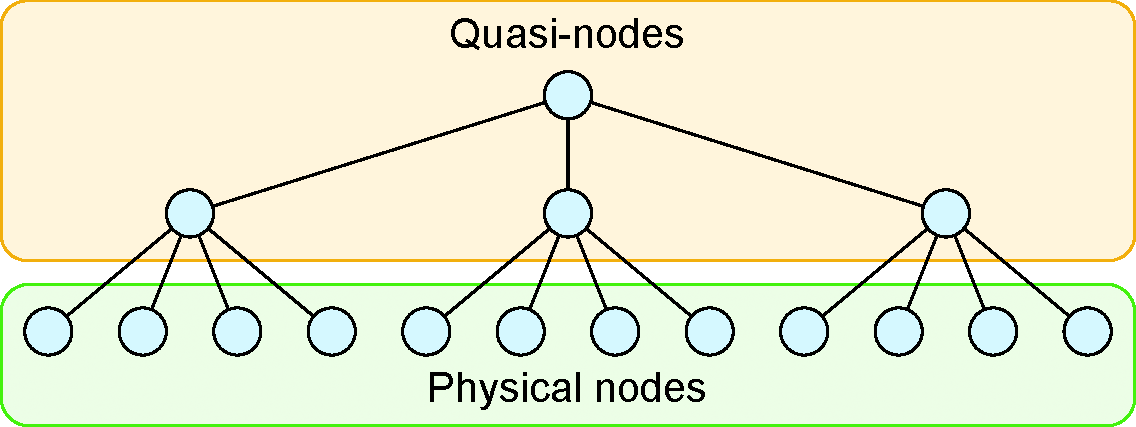
\includegraphics[width=\columnwidth]{figures/trust_hierarchy.pdf}
%	\caption{} \label{fig:trust_hierarchy}
%\end{figure}

\section{Consensus time}

DEFINITIONS

* Define consensus time of a message broadcast by node $i$ relative to a set of nodes $\mathcal{S}$,
\begin{align}
	\textsc{ConsensusTime}(i,\mathcal{S}) = \mathrm{median}(\{t_{i,j}\}_{j\in\mathcal{S}}),
\end{align}
where $t_{i,j}$ is the reported time-of-receipt of message $i$ by node $j$, and $\{t_{i,j}\}_{j\in\mathcal{S}}$ is the set of reported times-of-receipt of message $i$ by elements of $\mathcal{S}$.

* Use notation,
\begin{align}
	\vec{t}_{i,\mathcal{S}}   & = \{t_{i,j}\}_{j\in\mathcal{S}},\nonumber   \\
	\tilde{t}_{i,\mathcal{S}} & = \mathrm{median}(\vec{t}_{i,\mathcal{S}}).
\end{align}

* For any majority subset,
\begin{align}
	\mathcal{S}_+\subseteq\mathcal{S},\,\,|\mathcal{S}_+|>\frac{|\mathcal{S}|}{2},
\end{align}
we have,
\begin{align}
	\mathrm{min}(\vec{t}_{i,\mathcal{S}_+}) \leq \textsc{ConsensusTime}(i,\mathcal{S}) \leq \mathrm{min}(\vec{t}_{i,\mathcal{S}_+}).
\end{align}
Hence, the consensus-time of a set is bounded by any constituent majority.

* A majority of nodes reporting identical times-of-receipt,
\begin{align}
	t_{i,j}=t_{i,k} \;\forall\; j,k\in\mathcal{S}_+,
\end{align}
forces convergence of consensus-time,
\begin{align} \label{eq:ct_converge}
	\textsc{ConsensusTime}(i,\mathcal{S}) = t_{i,\mathcal{S}_+},
\end{align}
invariant under times reported by the minority, $\vec{t}_{i,\mathcal{S}_-}$.

PROTOCOL:
\begin{enumerate}
	\item All nodes $i\in\mathcal{S}$ report their times-of-receipt of a given message,
	      \begin{align}
		      \mathcal{B} \gets t_i,
	      \end{align}
	      and initialise their set of recognised compliant nodes as those whose timestamps subjectively arrived on time,
	      \begin{align}
		      \mathcal{S}_i^{(0)} = \{j\in\mathcal{S} \,|\, \textsc{ReceivedOnTime}_i(t_{j\to i})\}.
	      \end{align}
	      %	\item Reported $t_{i,j}$ are required to be received within a given window to comply with synchronicity. (talk about tau max constraint).
	      %	\item Under the latency profile nodes may have different subjective interpretations of which reported times they accept and hence different subjective understandings of consensus-time.
	\item Nodes $i$ record the arrival times of all timestamps announced by $j$ they recognise as compliant ($j\in\mathcal{S}_i$),
	      \begin{align}
		      \mathcal{B} \to \{t_{j\to i}\}_{j\in \mathcal{S}_i}.
	      \end{align}
	      and update their set of recognised compliant nodes accordingly,
	      \begin{align}
		      \mathcal{S}_i^{(n)} = \{j\in\mathcal{S}_i^{(n-1)} \,|\, \textsc{ReceivedOnTime}_i(t_{j\to i})\}.
	      \end{align}
	      With increasing $n$, subjective subsets of compliant nodes are non-expanding,
	      \begin{align}
		      \mathcal{S}_j^{(n)} & \subseteq \mathcal{S}_j^{(n-1)}.
	      \end{align}
	\item Nodes announce the set of received timestamps they deem compliant (for the $n$th round),
	      \begin{align}
		      \mathcal{T}_i^{(n)}(S_i^{(n)}) & = \{t_{j\to i}^{(n)}\}_{j\in S_i^{(n)}}, \nonumber \\
		      \mathcal{B}                    & \gets \mathcal{T}_i^{(n)}(S_i^{(n)}).
	      \end{align}
	      The median of $\mathcal{T}_i^{(n)}(S_i^{(n)})$ is node $i$'s subjective consensus-time.
	\item Nodes $i$ and $j$ mutually recognise the compliance of the set $\mathcal{S}_i \cap \mathcal{S}_j$. Node $i$ interprets the relative consensus-time implied by $j$ via their mutually recognised nodes,
	      \begin{align}
		      \mathcal{T}_{j\to i}^{(n)} = \mathcal{T}_j^{(n)}(\mathcal{S}_i^{(n)} \cap \mathcal{S}_j^{(n)}).
	      \end{align}
	      %	\item These exhibit pairwise convergence,
	      %		\begin{align}
	      %			\mathcal{T}_j^{(n)}(\mathcal{S}_i \cap \mathcal{S}_j).
	      %		\end{align}
	\item On a pairwise basis relative consensus-times are unambiguous.
	\item Nodes update their sets of timestamps to their new pairwise mutually recognised relative consensus-times,
	      \begin{align}
		      t_i^{(n)} = \mathrm{median}_j(\mathcal{T}_{j\to i}^{(n)}(\mathcal{S}_i \cap \mathcal{S}_j))
	      \end{align}
	\item (Repeat to 1): All nodes announce their updated timestampe,
	      \begin{align}
		      \mathcal{B} \gets t_i^{(n)}.
	      \end{align}
	\item When an majority of nodes $j$ report the same subjective understandings of consensus-time of $i$, all honest nodes necessarily converge (Eq.~\eqref{eq:ct_converge}).
	\item Failure to converge arises when different nodes have different subjective interpretations of consensus-time, which can only occur via minority timing manipulation. This is only possible if when,
	      \begin{align}
		      \mathcal{S}_j\neq \mathcal{S}_k, \, j,k\in \mathcal{S}_H.
	      \end{align}
	\item If a majority of reported updated times (i.e subjective consensus-times) are identical convergence has been reached: TERMINATE.
\end{enumerate}

* ??? TODO

To enforce synchronisation of the protocol compliance requires nodes' broadcast messages to satisfy timing constraints under majority vote. To establish majority vote outcomes on the timing of messages we introduce \emph{consensus time}, given by the median of the reported times of receipt of messages (Alg.~\ref{alg:consensus_time}).

\begin{algorithm}[H]
	\begin{algorithmic}
		\Function{ConsensusTime}{$\mathcal{C}$, \texttt{message}} $\to \mathbb{R}$
		\State $\texttt{times} \gets \{\textsc{TimeOfReceipt}(i,\texttt{message})$\}$_{i\in\mathcal{C}}$
		\State \Return \textsc{Median}(\texttt{times})
		\EndFunction
	\end{algorithmic}
	\caption{Consensus time of a broadcast message is given by the median of the times of receipt reported by nodes.} \label{alg:consensus_time}
\end{algorithm}

Consensus time exhibits the property that if for any majority of consensus nodes,
\begin{align}
	|t_i - \textsc{ConsensusTime}(\mathcal{C},\texttt{message})|	\leq \delta,
\end{align}
no reported $t_i$ for the remaining minority can shift consensus time by more than $\delta$, making consensus time robust against minority manipulation. Consensus time may therefore be utilised as an implied majority vote on nodes' timing compliance,
\begin{align}
	\textsc{MajorityVote}(\mathcal{C}, \textsc{Compliant}(\texttt{message})).
\end{align}
Let the worst-case network latencies be,
\begin{align}
	\tau_\mathrm{max} = \max_{i,j\in\mathcal{N}}(\tau_{i,j}),
\end{align}
where $\tau_{i,j}$ is the matrix of point-to-point latencies between nodes $i$ and $j$. A message broadcast at time $t_B$ will be received by all network nodes by at latest $t_B+\tau_\mathrm{max}$.
By majority vote, the latest time at which a message could have been broadcast is,
\begin{align}
	t_B \leq \textsc{ConsensusTime}(\mathcal{C},\texttt{message}) - \tau_\mathrm{max}.
\end{align}

Ensuring majority votes on consensus time are well-defined requires,
\begin{align}
	\delta \geq \frac{\tau_\mathrm{max}}{2}.
\end{align}

The possible values for the median of a set of numbers $\vec{t}=\{t_i\}_i$ is discretised, limited to being one of the values $t_i$ or the mean of two nearest ones, $(t_i+t_{i+1})/2$, where $t_{i+1}\geq t_i$ are ordered. If $\vec{t}$ are the times reported by a majority, consensus-time is similarly constrained.

Considering a set of parties with maximal dishonest minority, with $|\mathcal{N}_H|$ honest nodes and $|\mathcal{N}_D|=|\mathcal{N}_H|-1$ dishonest nodes, such that $|\mathcal{N}|=2\cdot|\mathcal{N}_H|-1$. Then we have,


* Let $\mathcal{S}_{j,k}$

* Consider an honest majority of nodes with different subjective


* Under an honest-majority assumption, if honest nodes

-

* For a network with honest majority

\begin{align}
	\mathrm{min}(\mathcal{N}_H)\leq\textsc{ConsensusTime}(\mathcal{N}_H) \leq \mathrm{max}(\mathcal{N}_H).
\end{align}
Including dishonest timestamps the inequality remains unchanged,
\begin{align}
	\mathrm{min}(\mathcal{N}_H)\leq\textsc{ConsensusTime}(\mathcal{N}) \leq \mathrm{max}(\mathcal{N}_H).
\end{align}
Given,
\begin{align}
	\mathrm{max}(\mathcal{N}_H) - \mathrm{min}(\mathcal{N}_H) \leq  \tau_\mathrm{max}.
\end{align}

If all honest nodes $\mathcal{N}_H$ report the same time their subjective consensus times converge (\mbox{$\delta\to 0$}) and cannot be manipulated by any minority tactic.

Consensus time may be subjective when nodes include timestamps from different sets of nodes, which may arise when dishonest nodes manipulate message timing such that their arrival times yield ambiguous inclusion.
\begin{align}
	\textsc{ConsensusTime}(\{\mathcal{C}\}_i) \neq \textsc{ConsensusTime}(\{\mathcal{C}\}_j),
\end{align}
for different subjective sets of timestamps to include, $\{\mathcal{C}\}_i$ and $\{\mathcal{C}\}_j$.

\subsubsection{Consensus-time convergence}

All nodes $i$ broadcast time-of-receipt of a message, $t_i^{(0)}$. Messages must be received within cutoff time $T_0$. Assume all honest nodes time-of-receipt are within cutoff. Dishonest nodes may manipulate their transmission timing to create subjective ambiguity in which timestamps are acknowledged by different nodes.

The consensus-time based only on honest nodes is bounded by,
\begin{align}
	t_H = \textsc{ConsensusTime}(\mathcal{N}_H),\nonumber \\
	\mathrm{min}(\mathcal{N}_H) \leq t_H\leq \mathrm{max}(\mathcal{N}_H).
\end{align}
For all nodes it is similarly bounded under honest majority, \mbox{$|\mathcal{N}_H|>|\mathcal{N}_D|$},
\begin{align}
	t_N = \textsc{ConsensusTime}(\mathcal{N}_H\cup \mathcal{N}_D),\nonumber \\
	\mathrm{min}(\mathcal{N}_H) \leq t_N\leq \mathrm{max}(\mathcal{N}_H)
\end{align}

Following the initial announcements of recorded arrival times, $t_i^{(0)}$, all nodes update their times to their subjectively observed consensus-times,
\begin{align}
	t_i^{(1)} = \textsc{ConsensusTime}(\mathcal{N}(i)),
\end{align}
where $\mathcal{N}(i)$ is the set of times observed by node $i$, which necessarily includes the reported times of all honest nodes, dictating common upper and lower bounds across all honest subjective $t_i^{(k)}$.

Updated times are announced to the network and employed for the subsequent round. The local update rule is recursively defined,
\begin{align}
	t_i^{(k)} = \textsc{ConsensusTime}(\mathcal{N}^{(k-1)}(i)).
\end{align}

In the absence of any dishonest nodes, all subjective $t_i^{(1)}$ will be equivalent and consensus-time convergence is achieved.

With only honest nodes, all $t_i^{(k)}$ converge after one round. Dishonest participants inhibit convergence by creating discrepancy between subjective consensus-times, but nonetheless remain bounded between the maximum and minimum of honest nodes. This creates a deadlock scenario where convergence is prevented.

%Under one-way drift, updated subjective consensus-times of honest nodes is bounded by,
%\begin{align}
%	t_i^{(k-1)} \leq t_i^{(k)} \leq \mathrm{max}(\mathcal{N}_H),
%\end{align}
%independent of minority tactic.

%Under this update rule honest nodes are unable to attain subjective consensus-times exceeding $\mathrm{max}(\mathcal{N}_H)$.

%After repeat iterations steady state amongst honest nodes is achieved once the majority of honest nodes report identical consensus-times. For $N_H$ honest nodes, if $k>N_H/2$ report identical updated times

We achieve convergence in consensus-time when subjective consensus-times are stable.

%\begin{align}
%	\textsc{MajorityVote}(\mathcal{C}, \textsc{TransmissionTime}(\texttt{message}))
%\end{align}

%\subsection{Design considerations}
%
%* Scaling in units of hashes and digital signatures. Computation is dominated by signing, requiring O(?). And hashes.
%
%* Multiple consensus' assigned to nodes (inward arrows) may be parallelised.